\documentclass[a4paper]{article}

\usepackage[english]{babel}
\usepackage[utf8]{inputenc}
\usepackage{amsmath}
\usepackage{graphicx}
\usepackage[colorinlistoftodos]{todonotes}
\usepackage{hyperref}
\usepackage{listings}
\usepackage[numbers]{natbib}

\usepackage{booktabs} % To thicken table lines



\title{Creating Customer Segments}

\author{Uirá Caiado}

\date{\today}

\begin{document}

\maketitle

\begin{abstract}
As pointed out by \cite{Udacity}, today many companies collect vast amounts of data on their clientele and have a strong desire to understand the meaningful relationships hidden in their customer base. In this project, I will apply unsupervised learning techniques on product spending data collected for consumers of a wholesale distributor in Lisbon, Portugal. My goal is to define how best segment their customers into distinct categories. Afterwards, the segmentation found will be compared with an additional labeling. Lastly, I will suggest ways that the segmentation could assist the wholesale distributor with future service changes.
\end{abstract}

%%%%%%%%%%%%%%%%%%%%%%%%%%%%%%%%%%%%%%%%%%%%%%%%%%%%%%%%%%%%%%%%%%%%%%%%%%%%%%%%%%%%%%%%
%% INTRODUCTION
%%%%%%%%%%%%%%%%%%%%%%%%%%%%%%%%%%%%%%%%%%%%%%%%%%%%%%%%%%%%%%%%%%%%%%%%%%%%%%%%%%%%%%%%

\section{Introduction}
\label{sec:introduction}
In this section, I will give some background about the problem addressed and the goal of the project.

\subsection{Some Background}
As stated by Udacity\footnote{Source: \url{https://goo.gl/i8TQwZ}}  and bla.

Bla bla bla.

\subsection{Getting Started}
bla bla bla

%%%%%%%%%%%%%%%%%%%%%%%%%%%%%%%%%%%%%%%%%%%%%%%%%%%%%%%%%%%%%%%%%%%%%%%%%%%%%%%%%%%%%%%%
%% DATA EXPLORATION
%%%%%%%%%%%%%%%%%%%%%%%%%%%%%%%%%%%%%%%%%%%%%%%%%%%%%%%%%%%%%%%%%%%%%%%%%%%%%%%%%%%%%%%%


\section{Data Exploration}
\label{sec:data_exploration}
In this section, I will begin exploring the data through visualizations and code to understand how each feature is related to the others. I will observe a statistical description of the dataset, consider the relevance of each feature, and select a few sample data points from the dataset which I will track through the course of this project.

\subsection{Basic Facts}
Let's go ahead and execute a basic description of the student dataset (Table \ref{tab:basicfacts}):

\begin{table}[ht]
\centering
\begin{tabular}{l|r}
 & Value \\\hline
Total number of students & 42 \\
Total number of students & 395 \\
Number of students who passed & 265 \\
Number of students who failed & 130 \\
Number of features & 30 \\
Graduation rate of the class & 67.09 \%

\end{tabular}
\caption{\label{tab:basicfacts}Facts About the Dataset.}
\end{table}

Bla

\subsection{Bla}
bla bla.

\begin{figure}[ht]
\centering
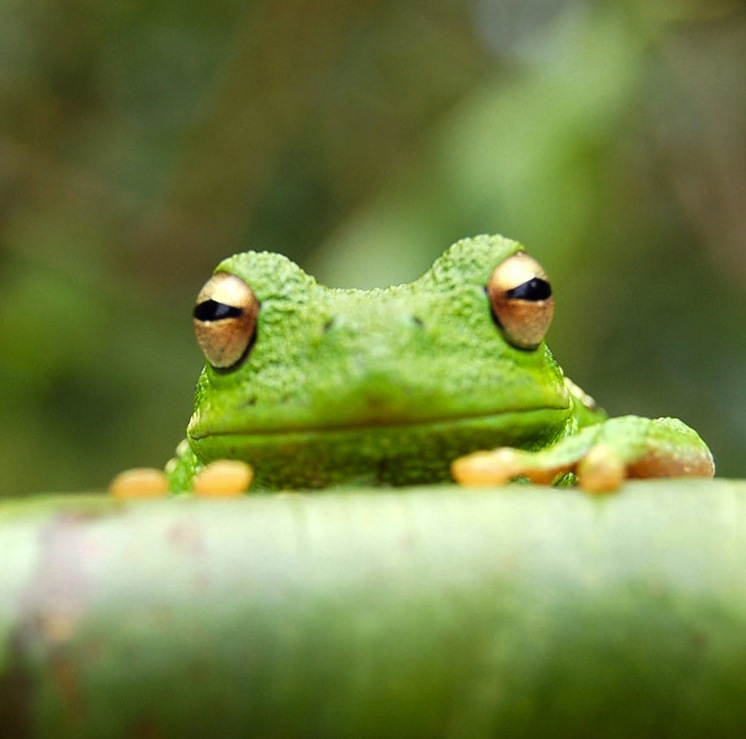
\includegraphics[width=0.45\textwidth]{figures/frog.jpg}
\caption{\label{fig:categorical}Categorical Data.}
\end{figure}

bla

%%%%%%%%%%%%%%%%%%%%%%%%%%%%%%%%%%%%%%%%%%%%%%%%%%%%%%%%%%%%%%%%%%%%%%%%%%%%%%%%%%%%%%%%
%% DATA PREPROCESSING
%%%%%%%%%%%%%%%%%%%%%%%%%%%%%%%%%%%%%%%%%%%%%%%%%%%%%%%%%%%%%%%%%%%%%%%%%%%%%%%%%%%%%%%%

\section{Data Preprocessing}
\label{sec:data_preprocessing}
In this section, I will preprocess the data to create a better representation of customers by performing a scaling on the data and detecting (and optionally removing) outliers. Preprocessing data is often times a critical step in assuring that results I obtain from my analysis are significant and meaningful.

%%%%%%%%%%%%%%%%%%%%%%%%%%%%%%%%%%%%%%%%%%%%%%%%%%%%%%%%%%%%%%%%%%%%%%%%%%%%%%%%%%%%%%%%
%% FEATURE TRANSFORMATION
%%%%%%%%%%%%%%%%%%%%%%%%%%%%%%%%%%%%%%%%%%%%%%%%%%%%%%%%%%%%%%%%%%%%%%%%%%%%%%%%%%%%%%%%

\section{Feature Transformation}
\label{sec:feature_transformation}
In this section I will use principal component analysis (PCA) to draw conclusions about the underlying structure of the wholesale customer data. Since using PCA on a dataset calculates the dimensions which best maximize variance, we will find which compound combinations of features best describe customers.


%%%%%%%%%%%%%%%%%%%%%%%%%%%%%%%%%%%%%%%%%%%%%%%%%%%%%%%%%%%%%%%%%%%%%%%%%%%%%%%%%%%%%%%%
%% CLUSTERING
%%%%%%%%%%%%%%%%%%%%%%%%%%%%%%%%%%%%%%%%%%%%%%%%%%%%%%%%%%%%%%%%%%%%%%%%%%%%%%%%%%%%%%%%

\section{Clustering}
\label{sec:clustering}
In this section, I will choose to use either a K-Means clustering algorithm or a Gaussian Mixture Model clustering algorithm to identify the various customer segments hidden in the data. I will then recover specific data points from the clusters to understand their significance by transforming them back into their original dimension and scale.


%%%%%%%%%%%%%%%%%%%%%%%%%%%%%%%%%%%%%%%%%%%%%%%%%%%%%%%%%%%%%%%%%%%%%%%%%%%%%%%%%%%%%%%%
%% CONCLUSION
%%%%%%%%%%%%%%%%%%%%%%%%%%%%%%%%%%%%%%%%%%%%%%%%%%%%%%%%%%%%%%%%%%%%%%%%%%%%%%%%%%%%%%%%

\section{Conclusion}
\label{sec:conclusion}


%%%%%%%%%%%%%%%%%%%%%%%%%%%%%%%%%%%%%%%%%%%%%%%%%%%%%%%%%%%%%%%%%%%%%%%%%%%%%%%%%%%%%%%%
%% REFLECTION
%%%%%%%%%%%%%%%%%%%%%%%%%%%%%%%%%%%%%%%%%%%%%%%%%%%%%%%%%%%%%%%%%%%%%%%%%%%%%%%%%%%%%%%%

\section{Reflection}
\label{sec:reflection}
Bla bla bla




\bibliographystyle{plain}
% or try abbrvnat or unsrtnat
\bibliography{bibliography/biblio.bib}
\end{document}
